\chapter{Diskussion der Ergebnisse}\label{cha:Robustheit}
Dieses Kapitel dient der Diskussion des in Kapitel \ref{cha:Regler} entworfenen Verkopplungsreglers. Dabei wird insbesondere auf die Erfüllung der in \ref{cha:Anforderungen} gestellten Anforderungen eingegangen. Der Entwurf wird zum einen am nominellen Modell, ohne Wirkung von Parameterschwankungen evaluiert und zum anderen für ein Modell, welches von Parameterunsicherheiten in Form von Abweichungen in der Flugzeugmasse beeinflusst wird. Dabei werden sowohl das um den Arbeitspunkt linearisierte Modell als auch das nichtlineare Modell verwendet. Abschließend werden in diesem Kapitel anhand des nominellen Modells strukturelle Erweiterungen erläutert, die die Robustheit bezüglich von außen auf die Flugzeuge wirkenden Störgrößen begünstigen.

\section{Ergebnisse des linearisierten Modells ohne Stellgrößenbeschränkung}
Zunächst soll nur das nominelle Modell betrachtet werden. In Abbildung \ref{fig:pzmap_controlled} ist dazu die Lage der Pol- und Nullstellen des geregelten Systems mit dem vorgegebenen Polgebiet dargestellt. In \ref{fig:pzmap_controlled_ohnezoom} ist gut zu erkennen, dass die invarianten Nullstellen des Systems durch entsprechende Platzierung von Eigenwerten kompensiert werden. Abbildung \ref{fig:pzmap_controlled_zoom} zeigt außerdem deutlich, dass alle Pole, wenn auch teilweise recht nah am Rand, innerhalb des vorgegebenen Polgebiets platziert werden.

\begin{figure}[h] % figure pzmap
	\centering
	\begin{subfigure}{.49\textwidth}
		\centering
		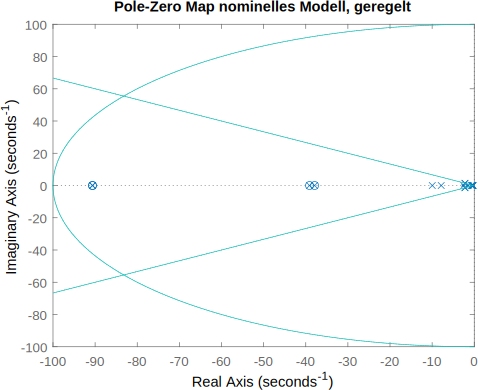
\includegraphics[width=\linewidth]{./Bilder/pzmap_controlled.eps}
		\caption{Vollständiges Polgebiet}
		\label{fig:pzmap_controlled_ohnezoom}
	\end{subfigure}
	\hfill
	\begin{subfigure}{.49\textwidth}
		\centering
		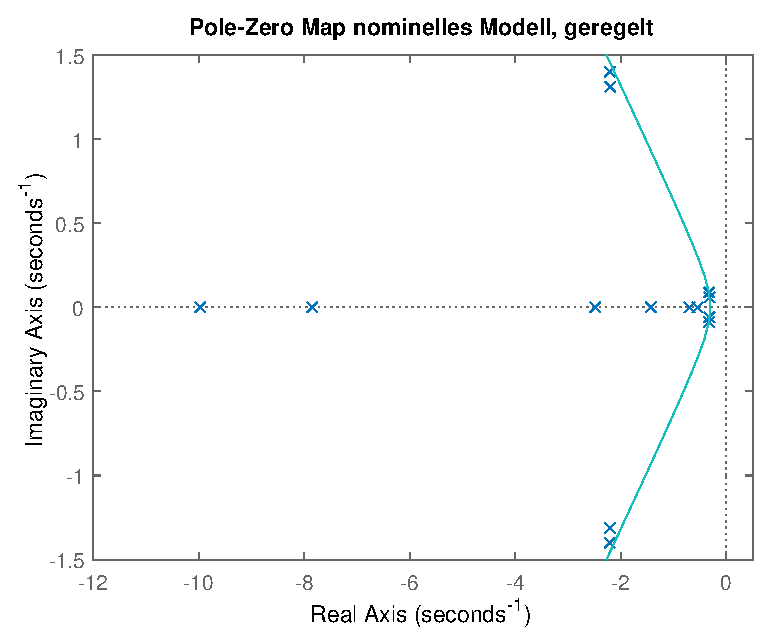
\includegraphics[width=\linewidth]{./Bilder/pzmap_controlled_zoom.eps}
		\caption{Polgebiet mit Fokus auf den Ursprung}
		\label{fig:pzmap_controlled_zoom}
	\end{subfigure}
	\caption{Pol-/ Nullstellendiagramm des geregelten Systems}
	\label{fig:pzmap_controlled}
\end{figure}

In den Abbildungen \ref{fig:outputs_linear_ohne_stellbesch} und \ref{fig:stellgr_linear_ohne_stellbesch} sind die Sprungantworten sowie die Stellgrößenverläufe des linearen Modells ohne Einfluss der Stellgrößenbeschränkungen dargestellt. Für die Führungsgrößen $v_1$ und $h_1$ wurden Sprünge von $\valunit{1}{m/s}$ respektive $\valunit{5}{m}$ ausgehend vom eigentlichen Arbeitspunkt vorgegeben. Für die beiden Eulerwinkel $\Phi_1$ und $\Theta_1$ wurden Sprünge von jeweils $\valunit{0.2}{rad}$ gewählt, was $\valunit{11.46}{\degree}$ entspricht. Bei Betrachtung der Sprungantworten in \ref{fig:outputs_linear_ohne_stellbesch} ist gut zu erkennen, dass die Verkopplung für alle Größen erfolgreich ist. Bei den ersten drei Verkopplungsausgängen liegt die Abweichung zwischen den beiden Flugzeugen im Bereich $1\eexp{-04}$ oder darunter, sodass dies als erfüllte Verkopplung anzusehen ist. Der Betrag der Differenz der beiden Höhen beläuft sich auf $\valunit{10}{m}$, was dem Abstand im Arbeitspunkt entspricht. Es ist außerdem zu erkennen, dass $v_1$ nach \valunit{2}{s} ohne Überschwingen und entkoppelt von den anderen Ausgängen des ersten Flugzeugs stationär genau einschwingt. Das gleiche gilt für $\Phi_1$ nach \valunit{5}{s}. Bei Betrachtung der Sprungantworten von $\Theta_1$ und $h_1$ fällt zudem auf, dass sich diese Größen gegenseitig beeinflussen, was durch die Wahl der Übertragungsmatrix zulässig ist. Die anderen Ausgangsgrößen von Flugzeug 1 werden dabei nicht beeinflusst. Diese beiden Größen benötigen jeweils etwa \valunit{15}{s} bis zum Erreichen des stationären Endwerts. Ein Sprung auf $\Theta_1$ führt dabei zu einem Höhenverlust von \valunit{15}{m} bevor die Höhe wieder auf ihrem Sollwert zurückgestellt wird, während ein Höhensprung lediglich einen sehr geringen Einfluss auf $\Theta_1$ hat. 

\begin{figure}[h] % figure nur linear ohne stellgrößenbeschränkung
	\centering
	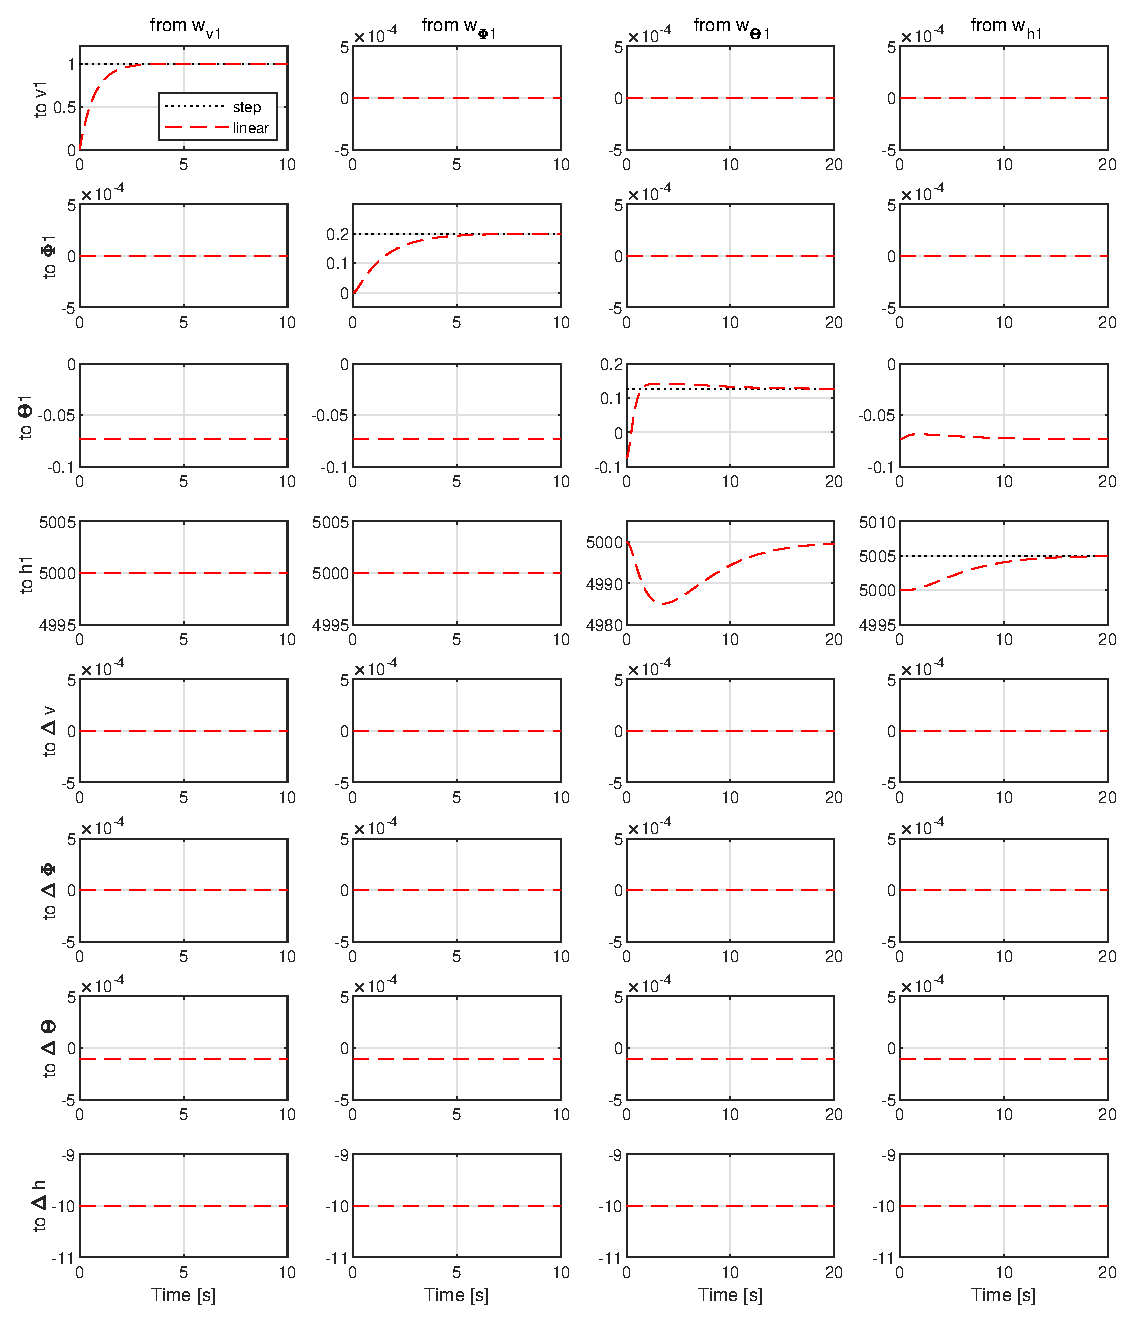
\includegraphics[width=\linewidth]{./Bilder/outputs_linear_ohne_stellbeschr.eps}
	\caption{Sprungantworten \textbf{ohne} Wirkung der Stellgrößenbeschränkung, lineares System}
	\label{fig:outputs_linear_ohne_stellbesch}
\end{figure}
\begin{figure}[h] % figure nur linear stellgrößen
	\centering
	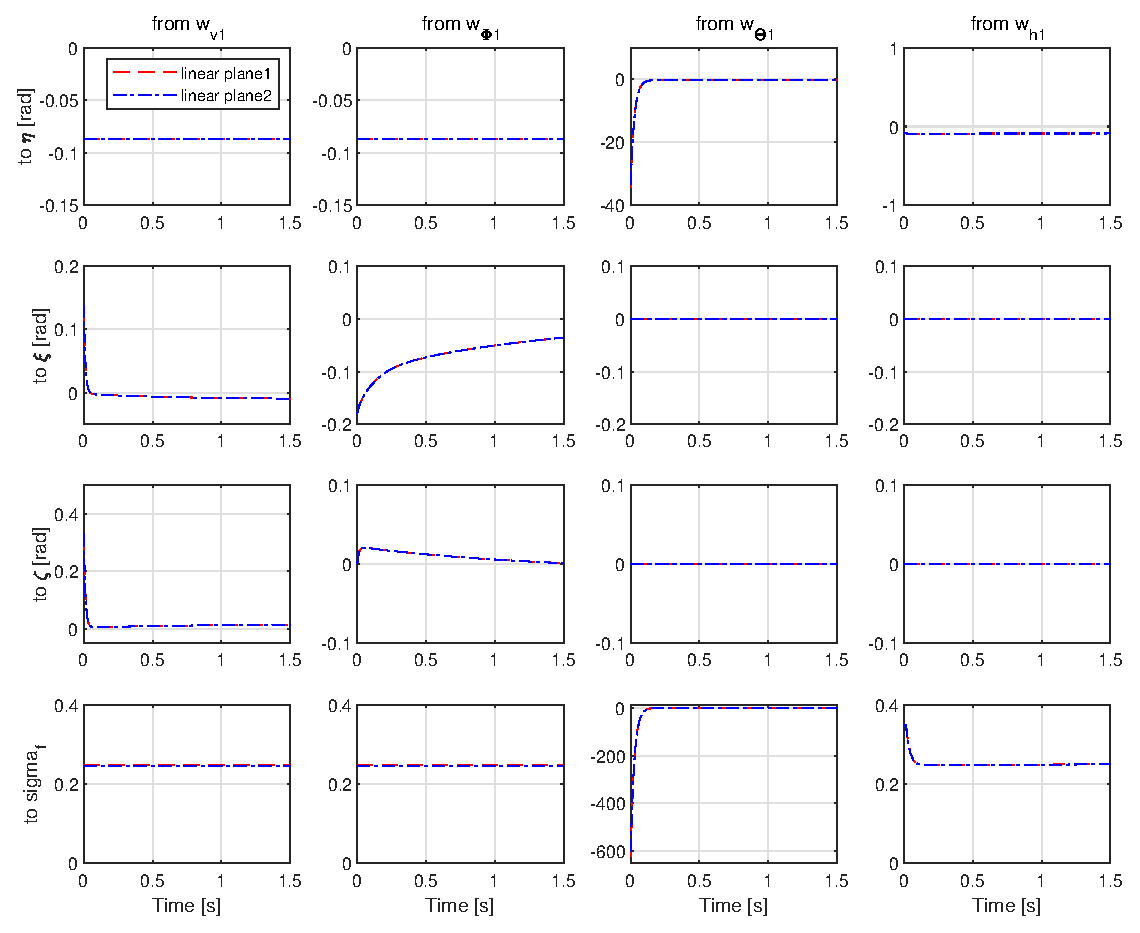
\includegraphics[width=\linewidth]{./Bilder/stellgr_linear_ohne_stellbeschr.eps}
	\caption{Stellgrößen \textbf{ohne} Wirkung der Stellgrößenbeschränkung, lineares System}
	\label{fig:stellgr_linear_ohne_stellbesch}
\end{figure}

Bei Betrachtung der Stellgrößenverläufe in Abbildung \ref{fig:stellgr_linear_ohne_stellbesch} fällt zunächst auf, dass diese für die beiden Flugzeuge nahezu identisch sind. Zudem lässt sich feststellen, dass beim Aufschalten von Führungssprüngen - mit Ausnahme von $\Theta_1$ - die Grenzen der Stellgrößen nicht verletzt werden. Bei $\Theta_1$ hingegen führt schon ein relativ geringer Sprung zu sehr hohen Stellgrößen, was unerwünscht ist. Bei Einführung der Stellgrößenbeschränkungen wird diese Eigenschaft zu unerwünschtem Systemverhalten führen. 

\section{Vergleich des linearen Modells mit dem nichtlinearen Modell unter Verwendung der Stellgrößenbeschränkungen}
Im Folgenden wird ebendieser Fall verdeutlicht. Die Abbildungen \ref{fig:outputs_linear_nlinear_mit_stellbeschr} und \ref{fig:stellgr_linear_nlinear_mit_stellbeschr} zeigen das Verhalten des linearen Modells im Vergleich mit dem nichtlinearen Modell unter Einfluss der Stellgrößenbeschränkung. Bei Betrachtung der dritten Spalte von Abbildung \ref{fig:stellgr_linear_nlinear_mit_stellbeschr} fällt zunächst auf, dass die Stellgrößen $\eta$ und $\tn{sigma}_f$ bei Anregung von $\Theta_1$ durch die Maximal- bzw. Minimalwerte begrenzt werden. Wie in Abbildung \ref{fig:outputs_linear_nlinear_mit_stellbeschr} führt dies zu unerwünschtem Systemverhalten (Änderung von $\Phi_1$ um mehr als \valunit{110}{\degree}), was darauf zurückzuführen ist, dass die Stellgrößenbeschränkung in diesem Fall wie eine Öffnung der Regelschleife wirkt. Es kann auf Zustandsänderungen nicht mehr sinngemäß reagiert werden, wodurch sich das System schnell vom Arbeitspunkt entfernt. Das Modell verliert damit für diesen Bereich seine Gültigkeit. Dieser Einfluss wirkt sich beim linearen Modell allerdings stärker aus als beim nichtlinearen Modell. Dies zeigt sich darin, dass die Verkopplung beim nichtlinearen Modell inbesondere bei der Höhe besser erreicht wird. Des Weiteren fällt auf, dass die erste und die vierte Spalte von Abbildung \ref{fig:outputs_linear_nlinear_mit_stellbeschr} mit denen aus Abbildung \ref{fig:outputs_linear_ohne_stellbesch} übereinstimmen. Daraus lässt sich zum einen schließen, dass für sprungförmige Anregungen auf die jeweiligen Eingänge $v_1$ und $h_1$ das lineare Modell und das nichtlineare Modell sehr gut übereinstimmen. Zum anderen lässt sich schlussfolgern, dass bei den entsprechenden Sprunghöhen die Stellgrößenbeschränkungen weder beim linearen noch beim nichtlinearen Modell verletzt werden. Auch beim nichtlinearen Modell wird die Verkopplung erreicht. Bei Betrachtung von Spalte zwei in Abbildung \ref{fig:outputs_linear_nlinear_mit_stellbeschr} ist deutlich erkennbar, dass das nichtlineare Modell bei einem Führungssprung von $\Phi_1$ vom linearen Modell abweicht. Während ein solcher Sprung beim linearen Modell lediglich $\Phi_1$ beeinflusst, so führt er beim nichtlinearen Modell auch zu einer Veränderung von $v_1$ und $h_1$. Dies liegt daran, dass das lineare Modell nur exakt im jeweiligen Arbeitspunkt gültig ist und die hier beaufschlagte Sollgröße zu einer Abweichung vom Arbeitspunkt führt, was sich in den nichtlinearen Systemgleichungen anders niederschlägt als in den linearisierten. Allerdings werden trotzdem die Stellgrößen eingehalten und die Verkopplung der beiden Flugzeuge erreicht.

\begin{figure}[h] % figure linear und nlinear mit stellgrößenbeschränkung
	\centering
	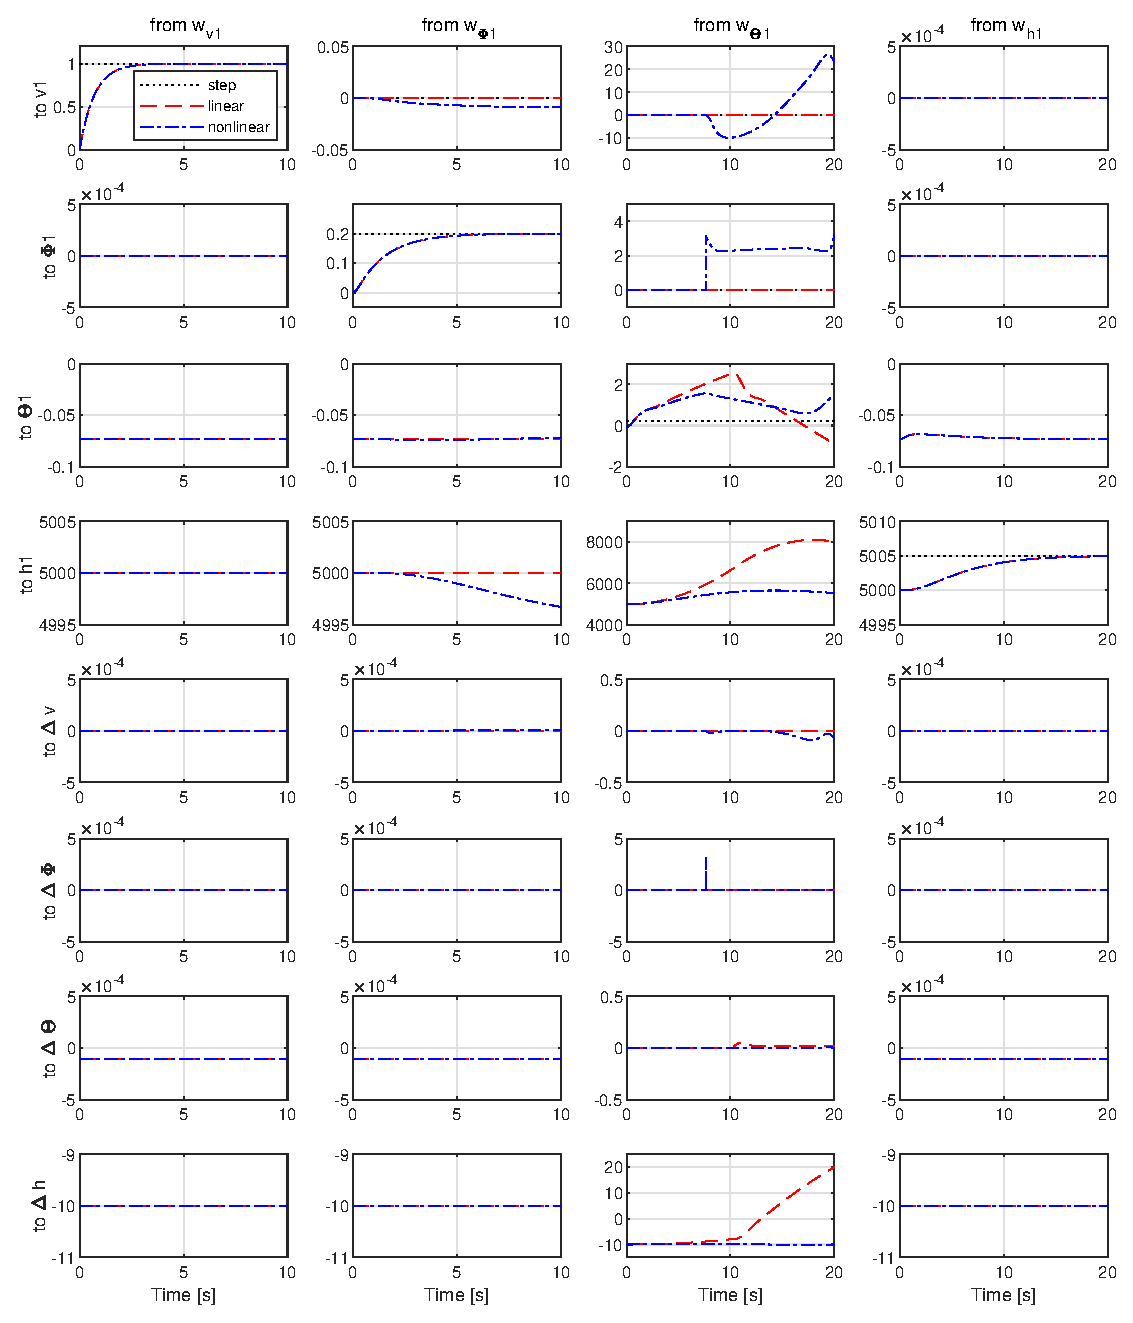
\includegraphics[width=\linewidth]{./Bilder/outputs_linear_nlinear_mit_stellbeschr.eps}
	\caption{Sprungantworten des linearen und nichtlinearen Modells \textbf{mit} Wirkung der Stellgrößenbeschränkung}
	\label{fig:outputs_linear_nlinear_mit_stellbeschr}
\end{figure}
\begin{figure}[h] % figure nur linear stellgrößen
	\centering
	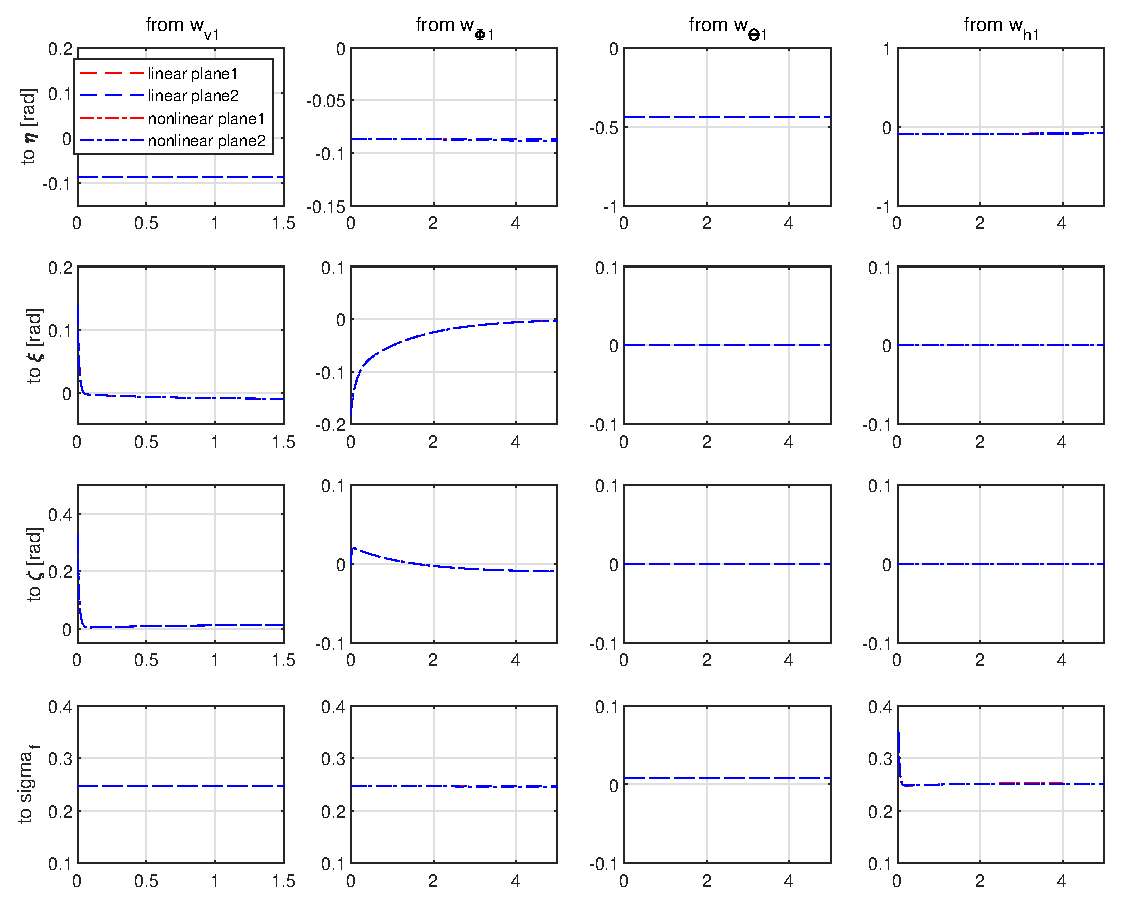
\includegraphics[width=\linewidth]{./Bilder/stellgr_linear_nlinear_mit_stellbeschr.eps}
	\caption{Stellgrößen des linearen und nichtlinearen Modells \textbf{mit} Wirkung der Stellgrößenbeschränkung}
	\label{fig:stellgr_linear_nlinear_mit_stellbeschr}
\end{figure}

Eine weitere Anforderung an die Regelung ist die Verkopplung der Flugzeugpositionen. Diese wird im Folgenden betrachtet und analysiert. Der Abstand der Flugzeuge ist in Abbildung \ref{fig:distance_xyz_nlinear} für das nichtlineare Modell dargestellt. Es ist gut zu erkennen, dass bei allen Sprunganregungen mit Ausnahme von $\Theta_1$ die Verkopplung der Flugzeugpositionen über den Simulationszeitraum gegeben ist. Der Abstand in Richtung der $y-$Achse beträgt null Meter. Für die $x-$Achse und die $z-$Achse beträgt der Abstand jeweils \valunit{10}{m}, was den gewünschten Werten entspricht. Die Darstellung über den relativ kurzen Zeitraum soll jedoch keine Einschränkung sein, da die Zustände nach Ablauf der Simulation bereits im eingeschwungenen Zustand sind. Das heißt, auch über einen längeren Zeitraum oder bei mehrfacher Anregung wäre die Verkopplung gewährleistet. Eine Anregung von $\Theta_1$ führt allerdings zu einer Abweichung der Werte von ihren Sollwerten und damit zu einem Verlust der Verkopplung der Positionen. 

Als Zwischenfazit lässt sich also festhalten, dass die Regelung prinzipiell dazu in der Lage ist, die Flugzeuge miteinander zu verkoppeln und auch die Entkopplung der Führungsgrößen von Flugzeug 1 wie gewünscht erreicht wird. Jedoch führen Führungssprünge beim Nickwinkel zu enorm hohen Stellgrößen, welche durch die Stellgrößenbeschränkung begrenzt werden und dadurch zum Verlust der gewünschten Eigenschaften führen. Die Regelung reagiert sehr sensitiv auf derartige Änderungen.

\begin{figure}[h] % figure distanz zwischen flugzeugen
	\centering
	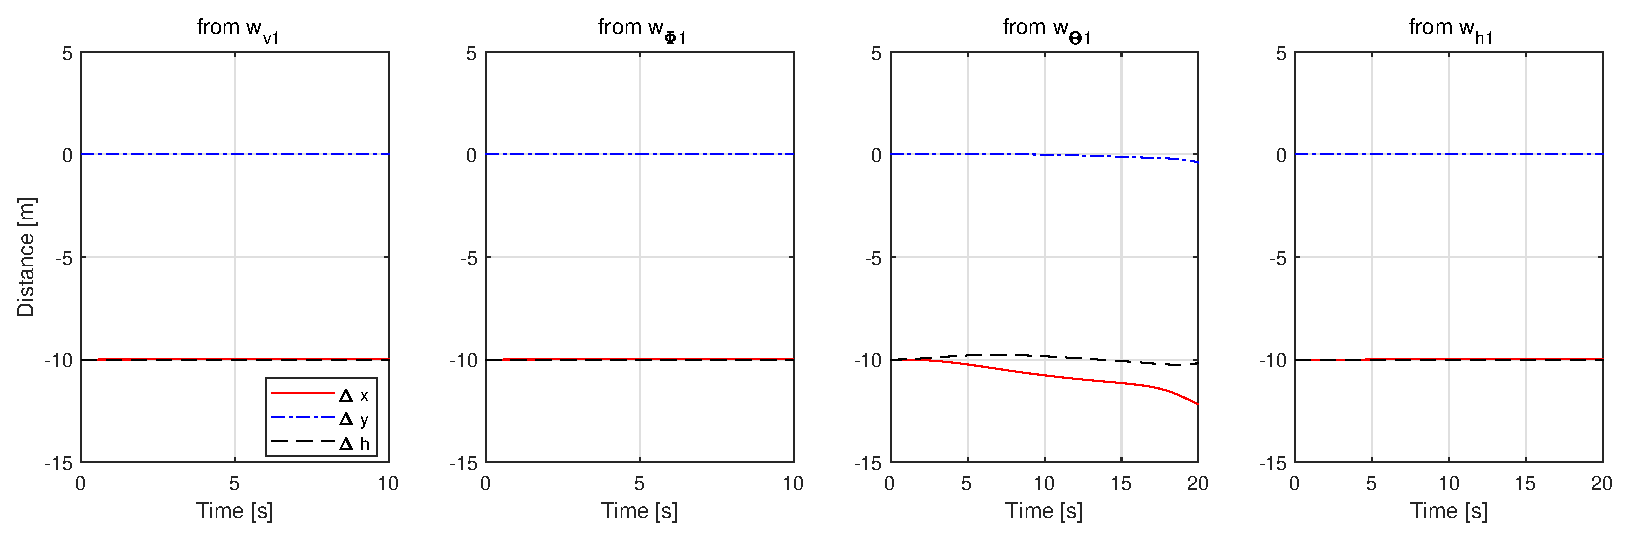
\includegraphics[width=\linewidth]{./Bilder/distance_xyz_nlinear.eps}
	\caption{Abstand der Flugzeuge zu einander am nichtlinearen Modell}
	\label{fig:distance_xyz_nlinear}
\end{figure}

\section{Ergebnisse Parameterschwankungen der Flugzeugmasse}
Nachdem nun das Systemverhalten des linearen und des nichtlinearen Modells miteinander verglichen und hinsichtlich der Anforderungen an die Regelung diskutiert wurde, soll nun der Einfluss von Parameterschwankungen in Form von unterschiedlichen Flugzeugmassen am nichtlinearen Modell analysiert werden. Die Parameterschwankung wirkt dabei so, dass zu Beginn der Betankung Flugzeug 1 (Tankflugzeug) zusätzliche zu seiner eigenen Masse die Masse des Treibstoffs transportiert, während Flugzeug 2 (betankte Flugzeug) nur seine eigene Masse transportiert. Es gilt also 
\begin{align}
	m_1 = m + t m_\tn{ks}, \qquad m_2 = m, \qquad \tn{mit} \, t\in\lbrack0,1\rbrack,
\label{eq:massmodel1}
\end{align}
wobei die Parameterschwankung über den Parameter $t$ zwischen 0 und \valunit{100}{\%} der gesamten Treibstoffmasse variiert werden kann.
Nach Abschluss der Betankung hat das Tankflugzeug die Treibstoffmasse an das zu betankende Flugzeug abgegeben und es gilt entsprechend
\begin{align}
	m_1 = m , \qquad m_2 = m + t m_\tn{ks}, \qquad \tn{mit} \, t\in\lbrack0,1\rbrack.
\label{eq:massmodel2}
\end{align}
Abbildung \ref{fig:pzmap_controlled_schwankung} zeigt das Pol-/ Nullstellendiagramm für das linearisierte nominelle System (Modell 1), das linearisierte System vor dem Betankungsvorgang entsprechend \ref{eq:massmodel1} (Modell 2) und das linearisierte System nach dem Betankungsvorgang entsprechend \ref{eq:massmodel2} (Modell 3). Durch die unterschiedlichen Massen ergeben sich leicht abweichende Arbeitspunkte und dadurch auch unterschiedliche Systemmatrizen. Bei Vorgabe der entsprechenden Größen zur Bestimmung des Arbeitspunktes für den Geradeausflug (siehe Kapitel [Referenz AP Trimming]) ändern sich durch die zusätzliche Masse die Größen $w, \Theta, \eta$ und $\tn{sigma}_f$. Bei voller Treibstoffmasse gilt im Arbeitspunkt
\begin{align*}
w_\tn{AP1} = \valunit{-9.3012}{m/s}, \quad \Theta_\tn{AP1} = \valunit{-0.0619}{rad}, \quad \eta_\tn{AP1} = \valunit{-0.0954}{rad}, \quad \tn{sigma}_{f\tn{AP1}} = 0.2254
\end{align*}
für das auf \valunit{5000}{m} fliegende Flugzeug 1 und 
\begin{align*}
w_\tn{AP2} = \valunit{-9.2834}{m/s}, \quad \Theta_\tn{AP2} = \valunit{-0.0618}{rad}, \quad \eta_\tn{AP2} = \valunit{-0.0955}{rad}, \quad \tn{sigma}_{f\tn{AP2}} = 0.2252
\end{align*}
für das auf \valunit{5010}{m} fliegende Flugzeug 2.
Abbildung \ref{fig:pzmap_controlled_schwankung} zeigt, dass auch für die Modelle 2 und 3, bei denen jeweils ein Flugzeug um \valunit{11.67}{\%} schwerer ist als im nominellen Modell, für welches der Regler ursprünglich ausgelegt wurde, werden die invarainten Nullstellen durch Eigenwerte kompensiert alle Eigenwerte liegen innerhalb des vorgegebenen Polgebiets.

\begin{figure}[h] % figure pzmap multimodell
	\centering
	\begin{subfigure}{.49\textwidth}
		\centering
		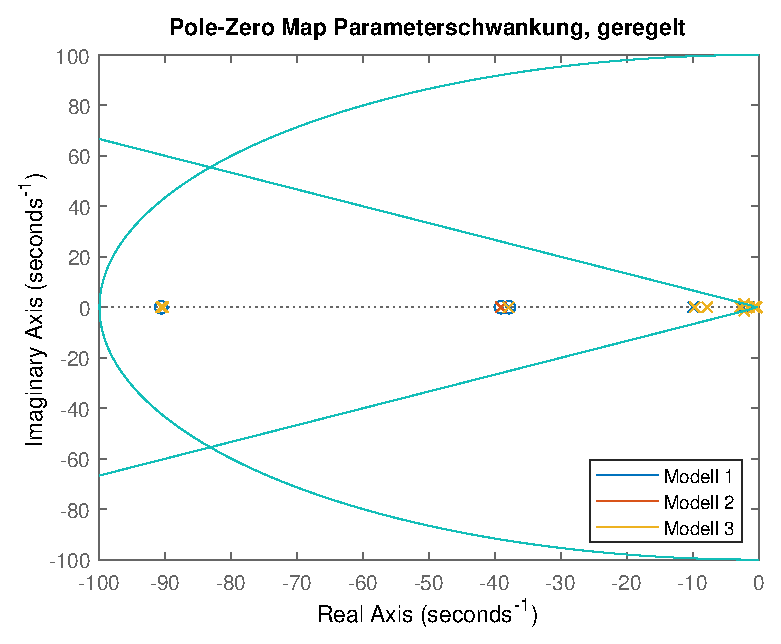
\includegraphics[width=\linewidth]{./Bilder/pzmap_controlled_schwankung.eps}
		\caption{Vollständiges Polgebiet}
		\label{fig:pzmap_controlled_schwankung_ohne_zoom}
	\end{subfigure}
	\hfill
	\begin{subfigure}{.49\textwidth}
		\centering
		\includegraphics[width=\linewidth]{./Bilder/pzmap_controlled_schwankung_zoom.eps}
		\caption{Polgebiet mit Fokus auf den Ursprung}
		\label{fig:pzmap_controlled_schwankung_zoom}
	\end{subfigure}
	\caption{Pol-/ Nullstellendiagramm der drei geregelten Systeme unter Einfluss von Parameterschwankungen für das nominelle System (Modell 1), das System vor dem Betankungsvorgang (Modell 2) und das System nach Abschluss der Betankung (Modell 3) mit $t=1$ (volle Tankladung).}
	\label{fig:pzmap_controlled_schwankung}
\end{figure}

Die Sprungantworten zu den Modellen 2 und 3 sowohl für den linearen als auch den nichtlinearen Fall sind in Abbildung \ref{fig:outputs_linear_nlinear_two_masses} dargestellt.

\begin{figure}[h] % figure sprungantworten zwei massenmodelle
	\centering
	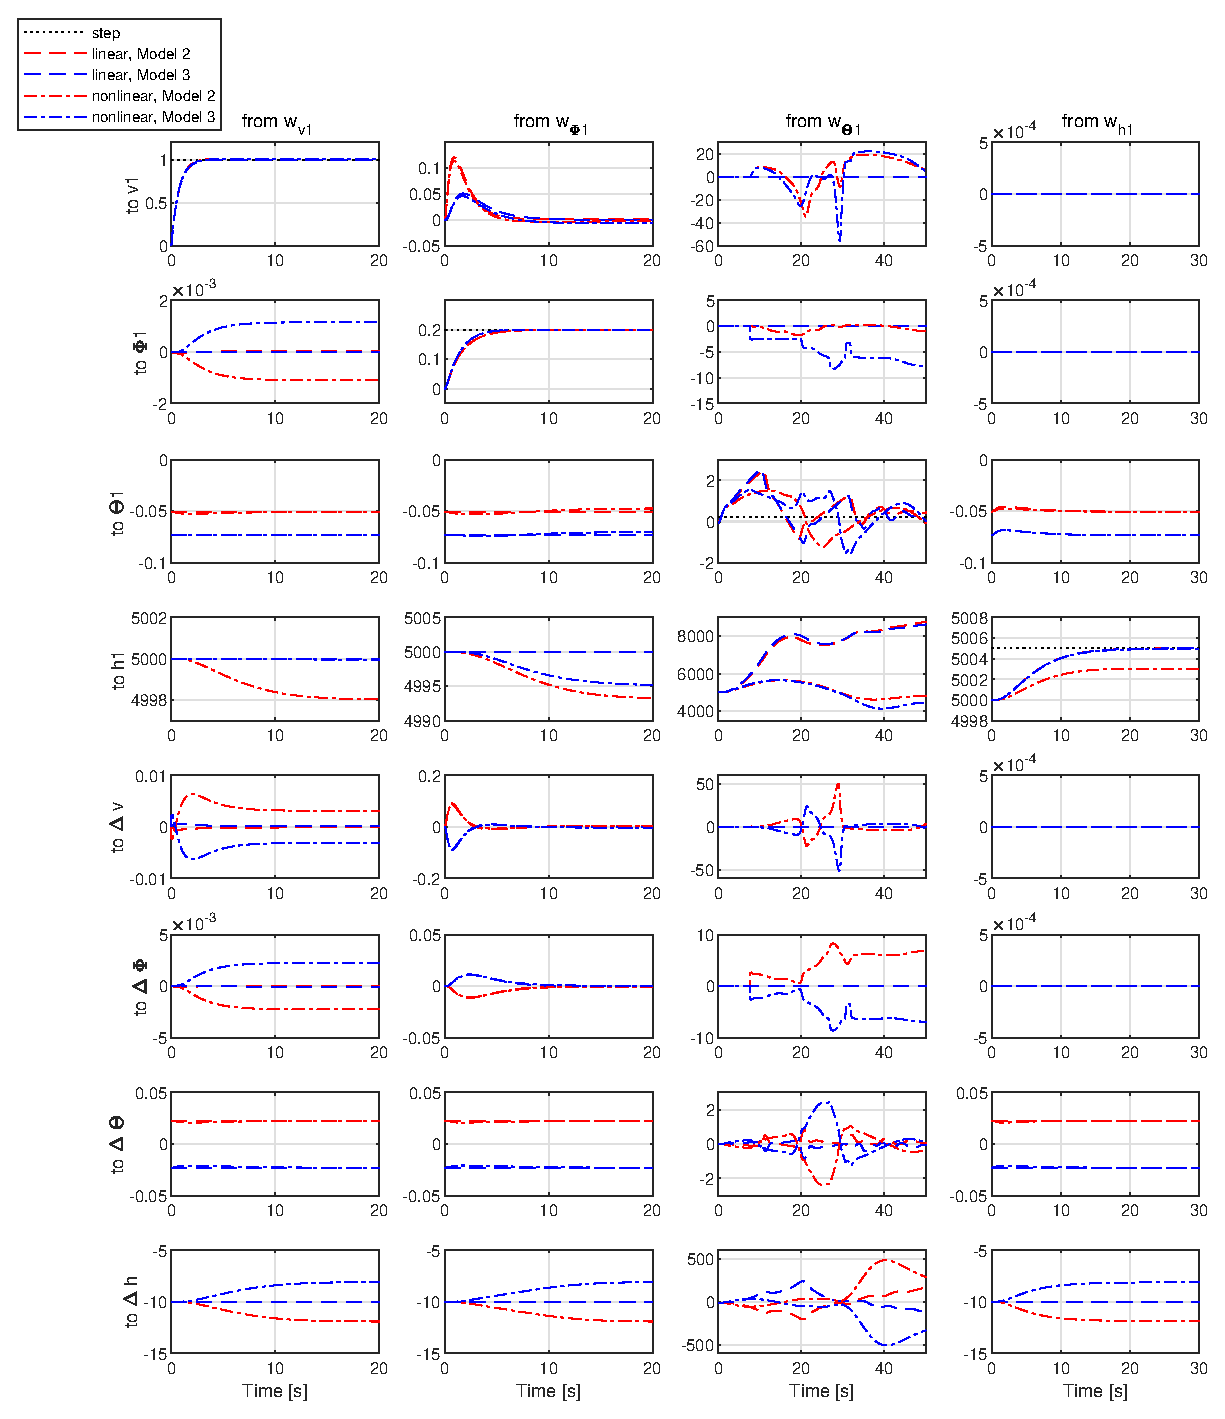
\includegraphics[width=\linewidth]{./Bilder/outputs_linear_nlinear_two_masses.eps}
	\caption{Sprungantworten der durch die Tankmasse beeinflussten Modelle 2 und 3 für das lineare und nichtlineare Modell}
	\label{fig:outputs_linear_nlinear_two_masses}
\end{figure}

Wie bereits beim nominellen Modell, führen auch bei den Modellen 2 und 3 Führungssprünge auf $\Theta_1$ zu instabilem Verhalten. Da die starke Sensitivität des Systems bezüglich Änderungen von $\Theta_1$ bereits umfassend erläutert wurde, soll an dieser Stelle nicht weiter darauf eingegangen werden. Es fällt auf, dass die Parameterschwankung der Masse großen Einfluss auf das Gesamtverhalten hat. Stationäre Genauigkeit ist bei Sprüngen auf $v_1$ und $\Phi_1$ bezüglich der jeweiligen Führungsgrößen nach wie vor gewährleistet. $v_1$ wird nun etwas stärker durch $\Phi_1$ beeinflusst, allerdings klingt dieser Einfluss schnell ab. Es lässt sich erkennen, dass die Sollhöhe beim nichtlinearen Modell nicht gehalten werden kann. Dies führt dazu, dass die Verkopplung der Höhen nicht mehr gewährleistet ist. Im Fall, dass Flugzeug 1 das schwerere Flugzeug ist, verliert es an Höhe, ohne dass Flugzeug 2 folgt, sodass der Abstand zwischen den beiden Flugzeugen größer wird. Im Fall, dass Flugzeug 2 bereits betankt wurde, ist es genau umgekehrt - die Flugzeuge nähern sich einander an. Dies gilt sowohl für Führungsgrößensprünge auf $v_1$ als auch auf $\Phi_1$. Außerdem entsteht im nichtlinearen Modell bei Sprüngen auf $v_1$ eine bleibende Abweichung für $\Delta v$ sowie $\Delta Phi$. Die Abweichung in $\Delta \Theta$, die in allen Fällen erkennbar ist, ist darauf zurück zu führen, dass die Flugzeuge aufgrund der unterschiedlichen Massen, wie zuvor erläutert, nun von einander abweichende Arbeitspunkte besitzen. Diese durch den Arbeitspunkt bedingte Abweichung lässt sich durch den Verkopplungsregler nicht ausregeln.
Führungssprünge bezüglich der Höhe haben keinerlei Einfluss auf $v_1$ und $\Phi_1$ und auch $\Theta_1$ wird nur leicht um den Arbeitspunkt herum ausgelenkt. Allerdings führt die Treibstoffmasse dazu, dass die stationäre Genauigkeit bezüglich der Höhe im nichtlinearen Modell verloren geht, sofern Flugzeug 1 das schwerere ist, da der Regler nicht dazu in der Lage ist diese Schwankung auszuregeln. Dies schlägt sich ebenfalls im verkoppelten Ausgang $\Delta h $ nieder. Ist Flugzeug 2 das schwerere, so wird der Sollwert bezüglich $h_1$ zwar stationär genau erreicht, jedoch gelingt es nicht das schwerere Flugzeug 2 nachzuführen, sodass auch in diesem Fall eine bleibende Höhendifferenz entsteht. 

Abbildung \ref{fig:distance_xyz_nlinear_twomassmodels} zeigt die Positionsdifferenz der beiden Flugzeuge für die Modelle 2 und 3. Es ist deutlich zu erkennen, dass die Regelung bei keinem der Modelle dazu in der Lage ist die Positionen miteinander zu verkoppeln. Dies liegt daran, dass die Parameterschwankung zu einer Abweichung des Modells vom nominellen Modell führen, für das die Regelung ausgelegt wurde. Da die Positionen nicht Bestandteil der in der Zustandsrückführung geregelten Zustände sind, hat die Regelung keine Möglichkeit auf Positionsdifferenzen zu reagieren. Abweichungen in der Geschwindigkeit und den Kurswinkeln $\gamma$ und $\chi$ werden aufintegriert, ohne darauf Einfluss nehmen zu können. Damit lässt sich als Abschluss dieses Abschnitts festhalten, dass die Verkopplungsregelung, so wie sie in dieser Arbeit ausgelegt wurde, den Einfluss der Parameterschwankung in der Flugzeugmasse nicht ausregeln kann. Bei Abweichung vom für die Reglerauslegung gültigen Modell, ist die Verkopplung der Flugzeuge nicht mehr gewährleistet. Die Robustheit gegenüber derartigen Schwankungen ist nicht gegeben.

\begin{figure}[h] % figure positionsdifferenz zwei massenmodelle
	\centering
	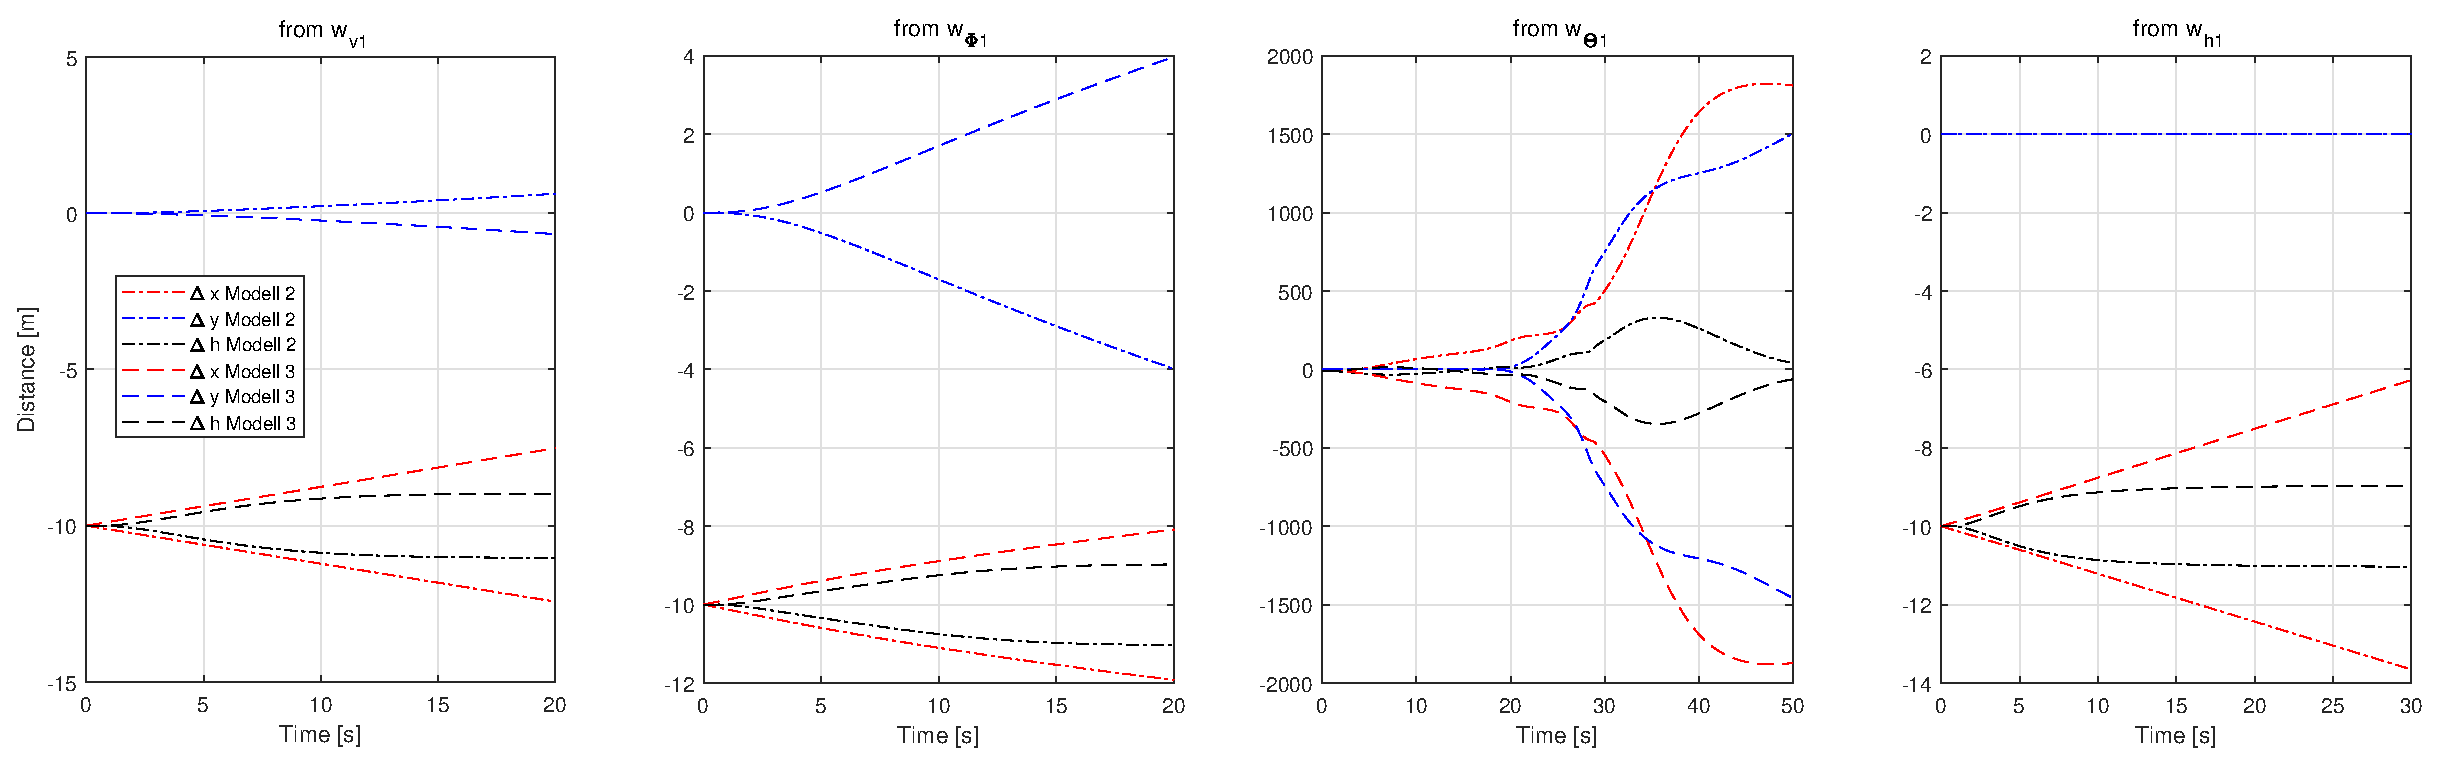
\includegraphics[width=\linewidth]{./Bilder/distance_xyz_nlinear_twomassmodels.eps}
	\caption{Abstand der Flugzeuge für die durch die durch die Massenschwankung beeinflussten nichtlinearen Modelle}
	\label{fig:distance_xyz_nlinear_twomassmodels}
\end{figure}

\section{Strukturelle Erweiterung für das nominelles Modell}
Neben Parameterschwankungen können auch andere Störfaktoren das Systemverhalten beeinflussen. Äußere Störeinflüsse, die zum Beispiel in Form von Wind in das System eingreifen, können dazu beitragen, dass das Systemverhalten instabil wird. Daher sollten diese durch die Regelung ausgeregelt werden. Als Modell wird das in \Simulink implementierte Windmodell "Discrete Wind Gust Model" verwendet, welches Windböen bezüglich der drei körperfesten Geschwindigkeitsachsen eines Flugzeugs erzeugt. Die Windböen werden als sprungförmige Stögrößen modelliert, welche direkten Einfluss auf die Geschwindigkeiten des Flugzeugs nehmen. Um sprungförmige Störgrößen stationär genau ausregeln zu können, muss der Regelkreis vor dem Einfluss der Störgröße einen I-Anteil besitzen [Referenz Föllinger o.ä]. Da dies durch den Verkopplungsregler nicht gewährleistet ist, wird im Folgenden zusätzlich zum Zustandsregler eine Ausgangsrückführung für die Führungsgrößen von Flugzeug 1 ausgelegt, die diese stationäre Genauigkeit bezüglich des Windeinflusses sicherstellen soll. Abbildung \ref{fig:blockschaltbild_unterlagerung} zeigt das Blockschaltbild der erweiterten Regelung. Für jeden der vier Führungsübertragungspfade 
\begin{align*}
	v_1 \rightarrow v_1, \qquad \Phi_1 \rightarrow \Phi_1, \qquad \Theta_1 \rightarrow \Theta_1, \qquad h_1 \rightarrow h_1 
\end{align*}
wird ein Regler mit einem I-Anteil so entworfen, dass vorhandene Null- und Polstellen, falls diese stabil sind, durch Hinzufügen zusätzlicher Null- und Polstellen, kompensiert werden. Der I-Anteil sorgt dafür, dass die Windstörungen stationär genau ausgeregelt werden können. Die Verstärkungsfaktoren der einzelnen Regler werden so gewählt, dass die hinzugefügten Polstellen möglichst den ursprünglichen entsprechen, sodass die Dynamik des äußeren Regelkreises der des inneren Regelkreises entspricht. Die Regler werden anhand des nominellen Modells entworfen, da nur für dieses die Verkopplung erreicht wurde.
\tikzstyle{block} = [draw, rectangle, 
minimum height=3em, minimum width=4em]
\tikzstyle{sum} = [draw, circle, node distance=1cm]
\tikzstyle{input} = [coordinate]
\tikzstyle{output} = [coordinate]
\tikzstyle{pinstyle} = [pin edge={to-,thin,black}]

\begin{figure}[h]
\centering
\begin{tikzpicture}[auto, node distance=3cm,>=latex']
% We start by placing the blocks
\node [input, name=input] {};
\node [sum, right of=input] (sum1) {};
\node [block, right of=sum1] (pidt_regler) {PIDT-Regler};
\node [block, right of=pidt_regler, pin={[pinstyle]above:Wind},
node distance=4cm] (system) {Verkoppeltes System};
\node [output, right of=system] (output) {};


% Once the nodes are placed, connecting them is easy. 
\draw [draw,->] (input) -- node {$\underline{w_1}$} (sum1);
\draw [->] (sum1) -- node {$\underline{e}$} (pidt_regler);
\draw [->] (pidt_regler) -- node {$\Delta\underline{w}_1$} (system);
\draw [->] (system) -- node [name=y] {$\underline{y}_1$}(output);
\draw [->] (y.south)  -- ++(0,-1.5cm) -| node[pos=0.99, right] {$-$} (sum1);
\end{tikzpicture}
\caption{Strukturbild der unterlagerten Regelung für das verkoppelte System.}
\label{fig:blockschaltbild_unterlagerung}
\end{figure}

\todo{Übertragungsfunktionen}
\todo{PID-Regler einführen}
\todo{Sprungantowrten zeigen}
\todo{blcokschaltbild unterlagerung}
\subsection{Ergebnisse Windeinfluss nominelles Modell}
\todo{srpungantowrten, zustaände wenn Windeinfluss}
